% Go into a lot of detail on how our prototype works right now, include photographs

\subsection{Functional Prototype}
The prototype consists of weight sensor readings sent to an HTTP server via POST requests. The web application displays the latest measurements in a simple dashboard, allows users to calibrate the empty/full weights of the water pitcher, and has a notification feature that works on web browsers.

\subsubsection{Hardware}
The plates used above and below the load cell are made for functional prototype purposes to fit the need of measure weight readings rather than
handling various water filter pitchers. Temporary HTTP server made to display and mimick how data is shown/handled.

\subsubsection{Web Application}
The current web application uses a clean, single-page dashboard layout. It is currently hosted at \url{https://cse123a-project-6a3s.vercel.app/}. It presents a water level percentage, a visual water-level indicator, 
and status text that communicates whether the pitcher has sufficient water. Additional metadata such as recent update information is shown to test and verify that data is being correctly received and displayed.\\

\begin{figure}[H]
\begin{center}
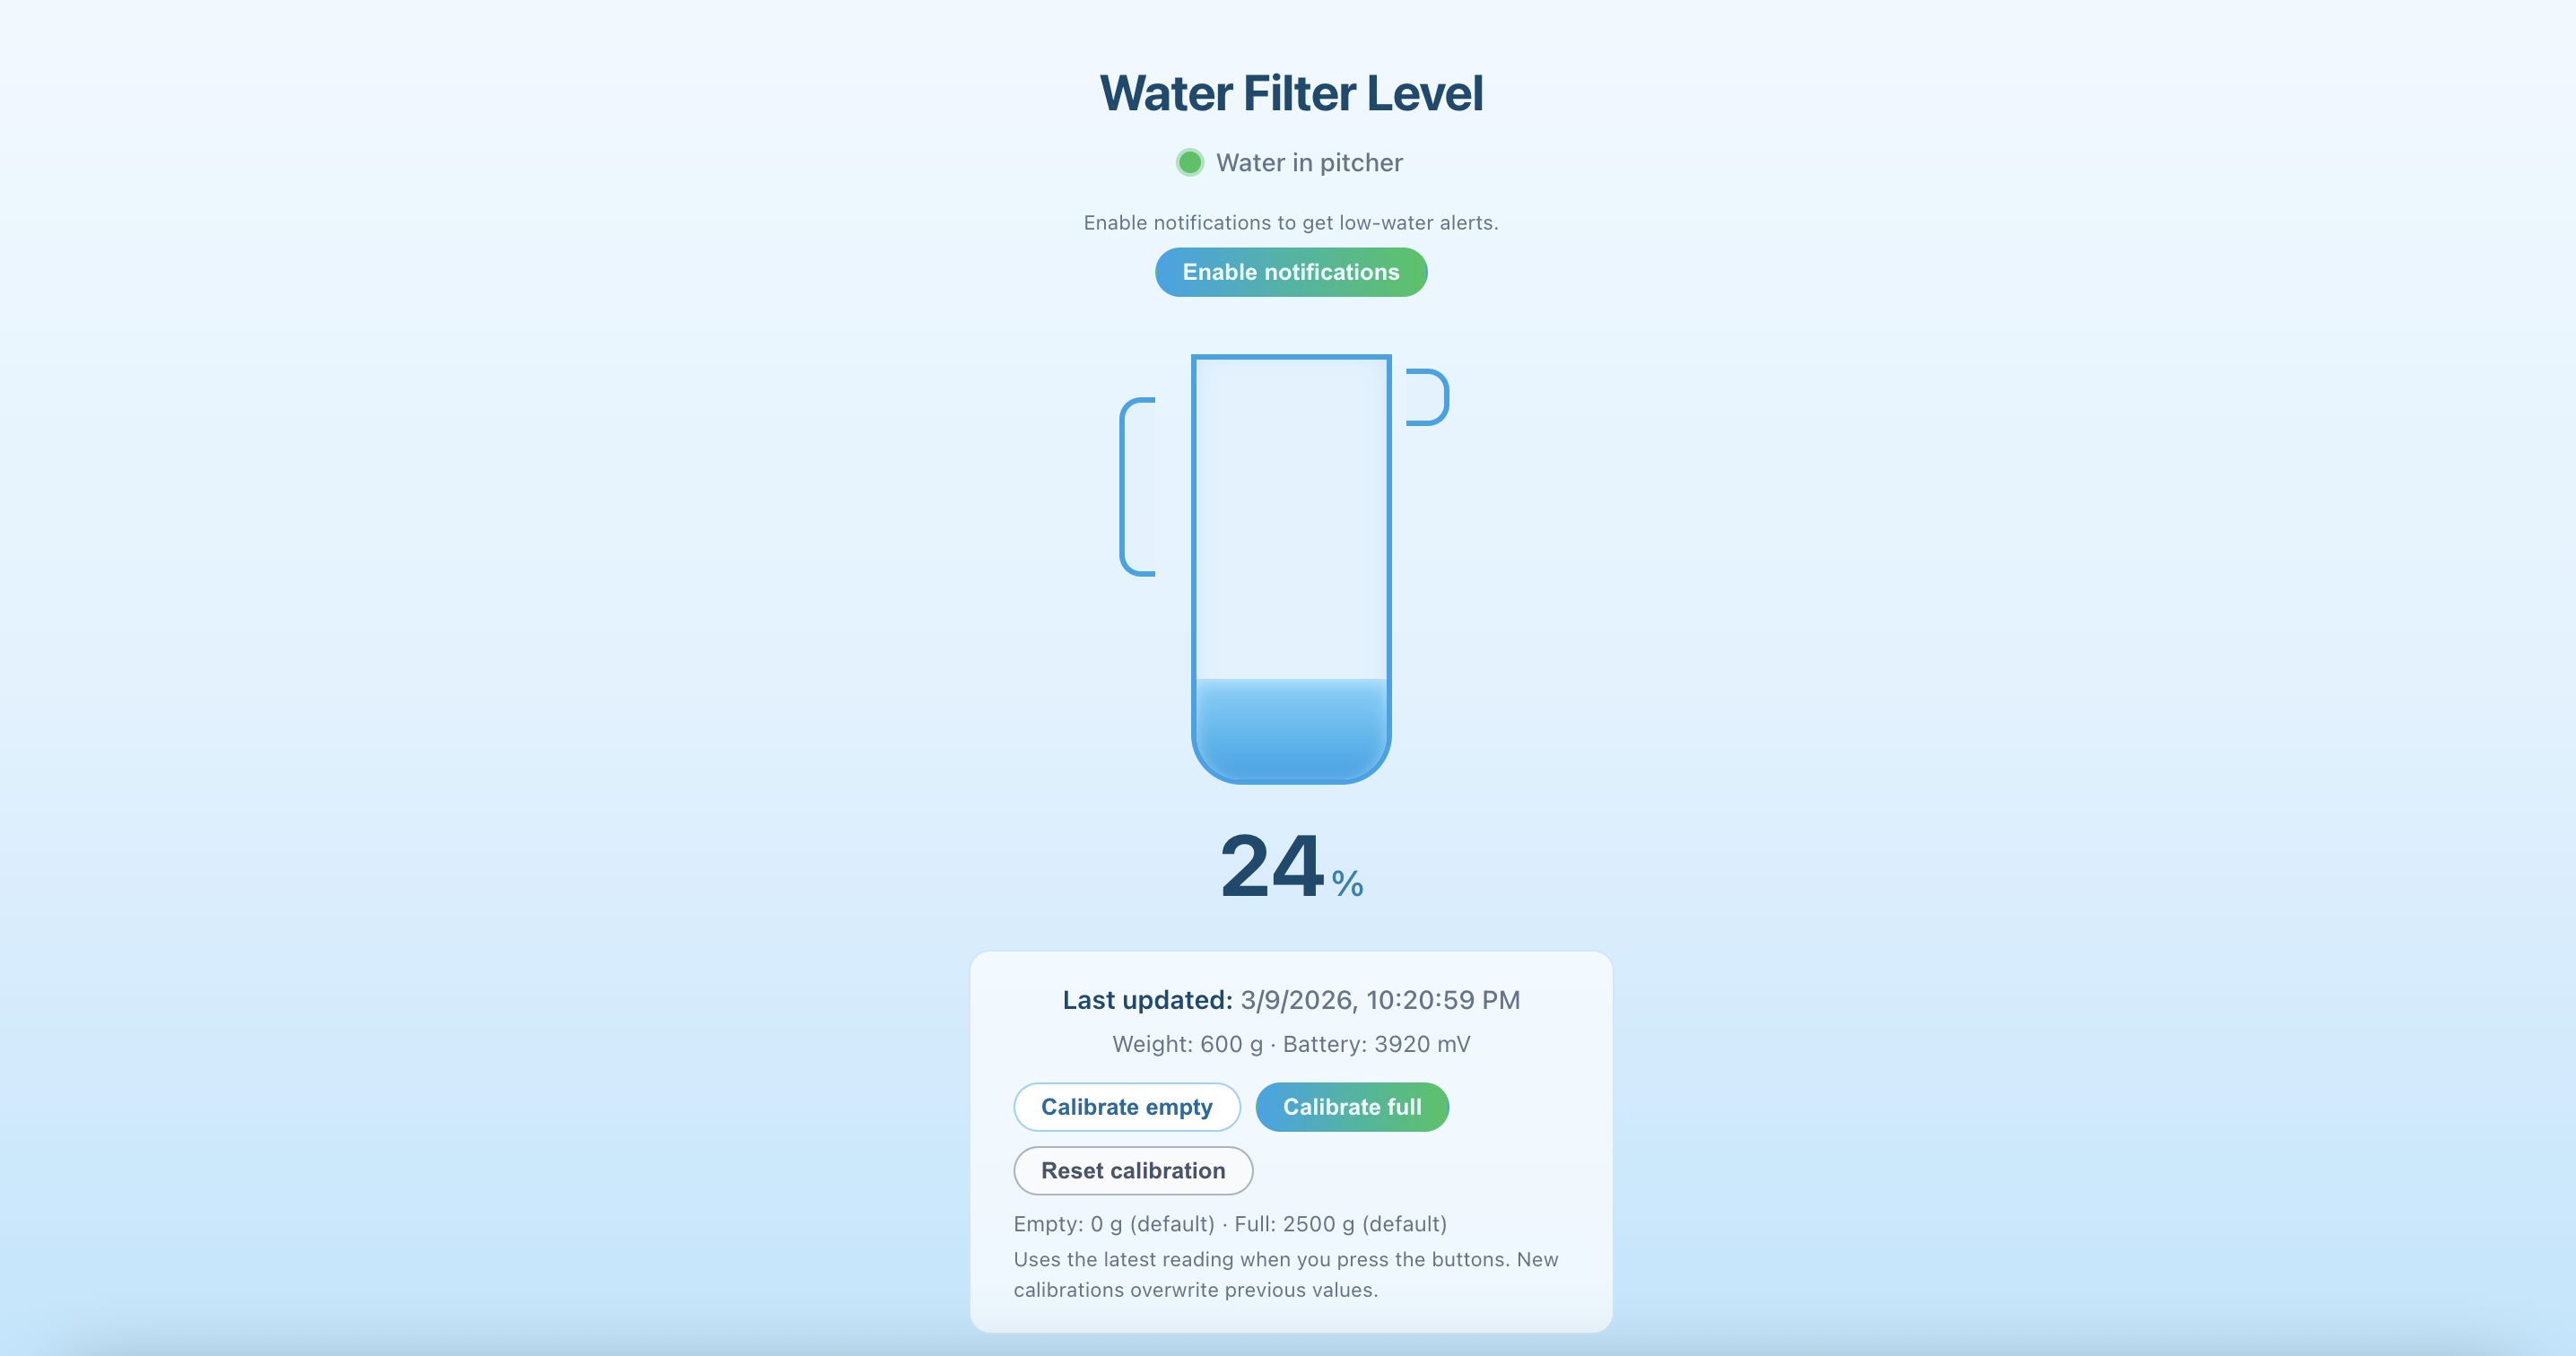
\includegraphics[width=0.75\textwidth]{sections/images/web_app_prototype.png}
\caption{Current Web Application Prototype Interface}
\label{web_app_prototype_eval}
\end{center}
\end{figure}

\noindent The web application works as follows:
\begin{enumerate}
	\item The ESP32 sends a new sensor reading to the server.
	\item The server stores the reading and makes it available to the dashboard.
	\item The dashboard fetches the latest value and updates the displayed percentage and water-level visual.
    \item Users can calibrate the system by pressing "Calibrate empty" when the latest value is an empty pitcher and "Calibrate full" when the latest value is a full pitcher.
	\item If the value is below the low-water threshold, the app sends a refill alert to users who enabled notifications.
\end{enumerate}

\begin{figure}[H]
\begin{center}
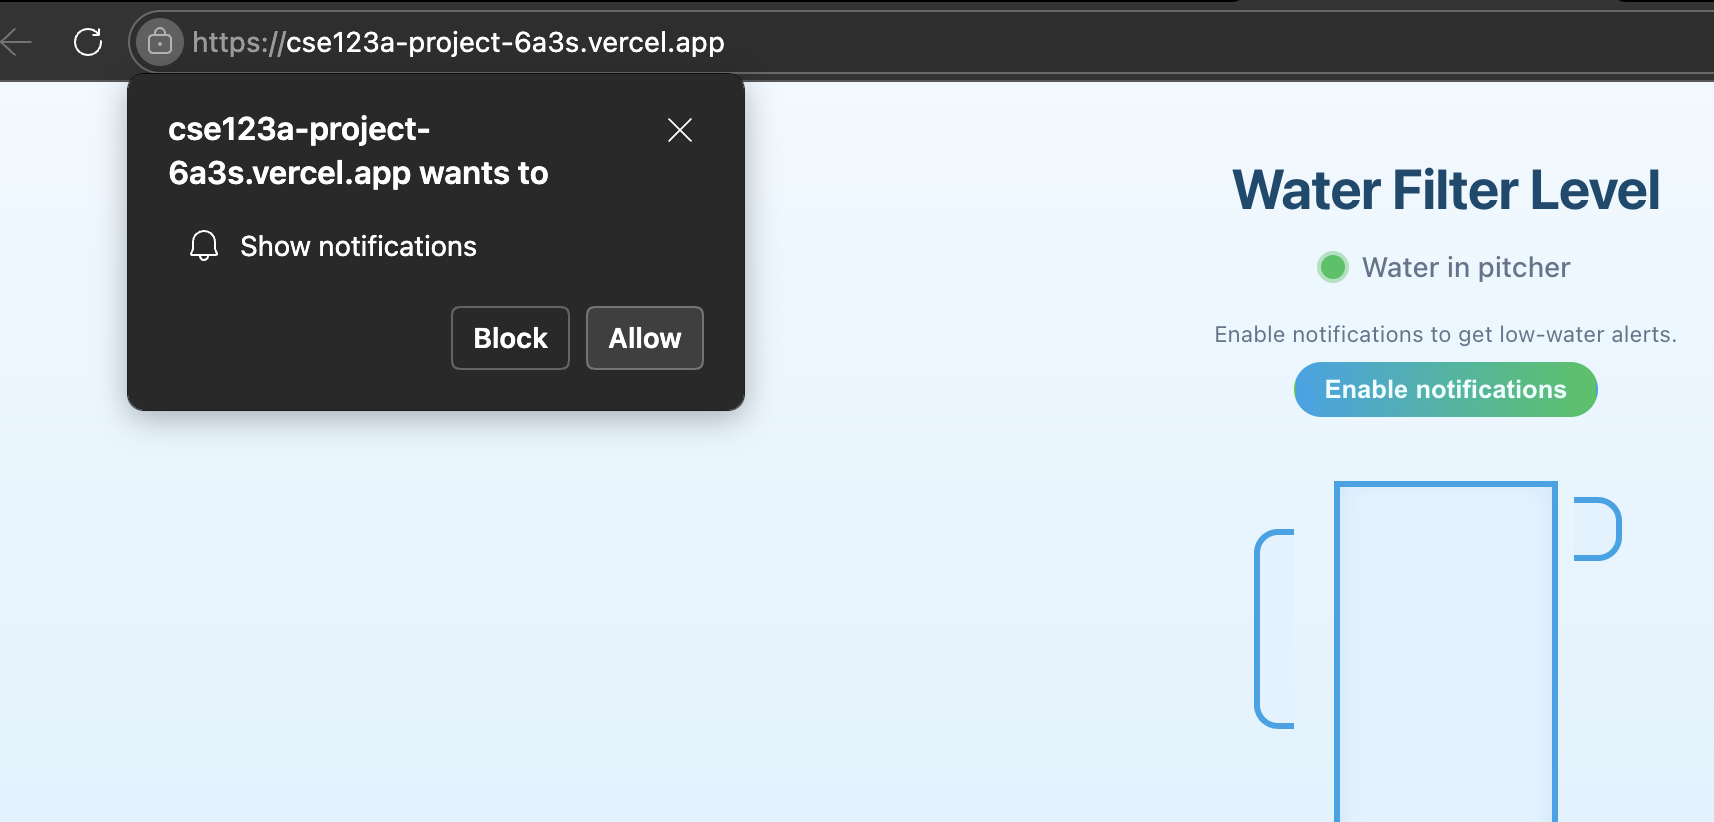
\includegraphics[width=0.75\textwidth]{sections/images/web_app_enable_notif_prompt.png}
\caption{Web Application Notification Permission Prompt}
\label{web_app_enable_notif_prompt_eval}
\end{center}
\end{figure}

\begin{figure}[H]
\begin{center}
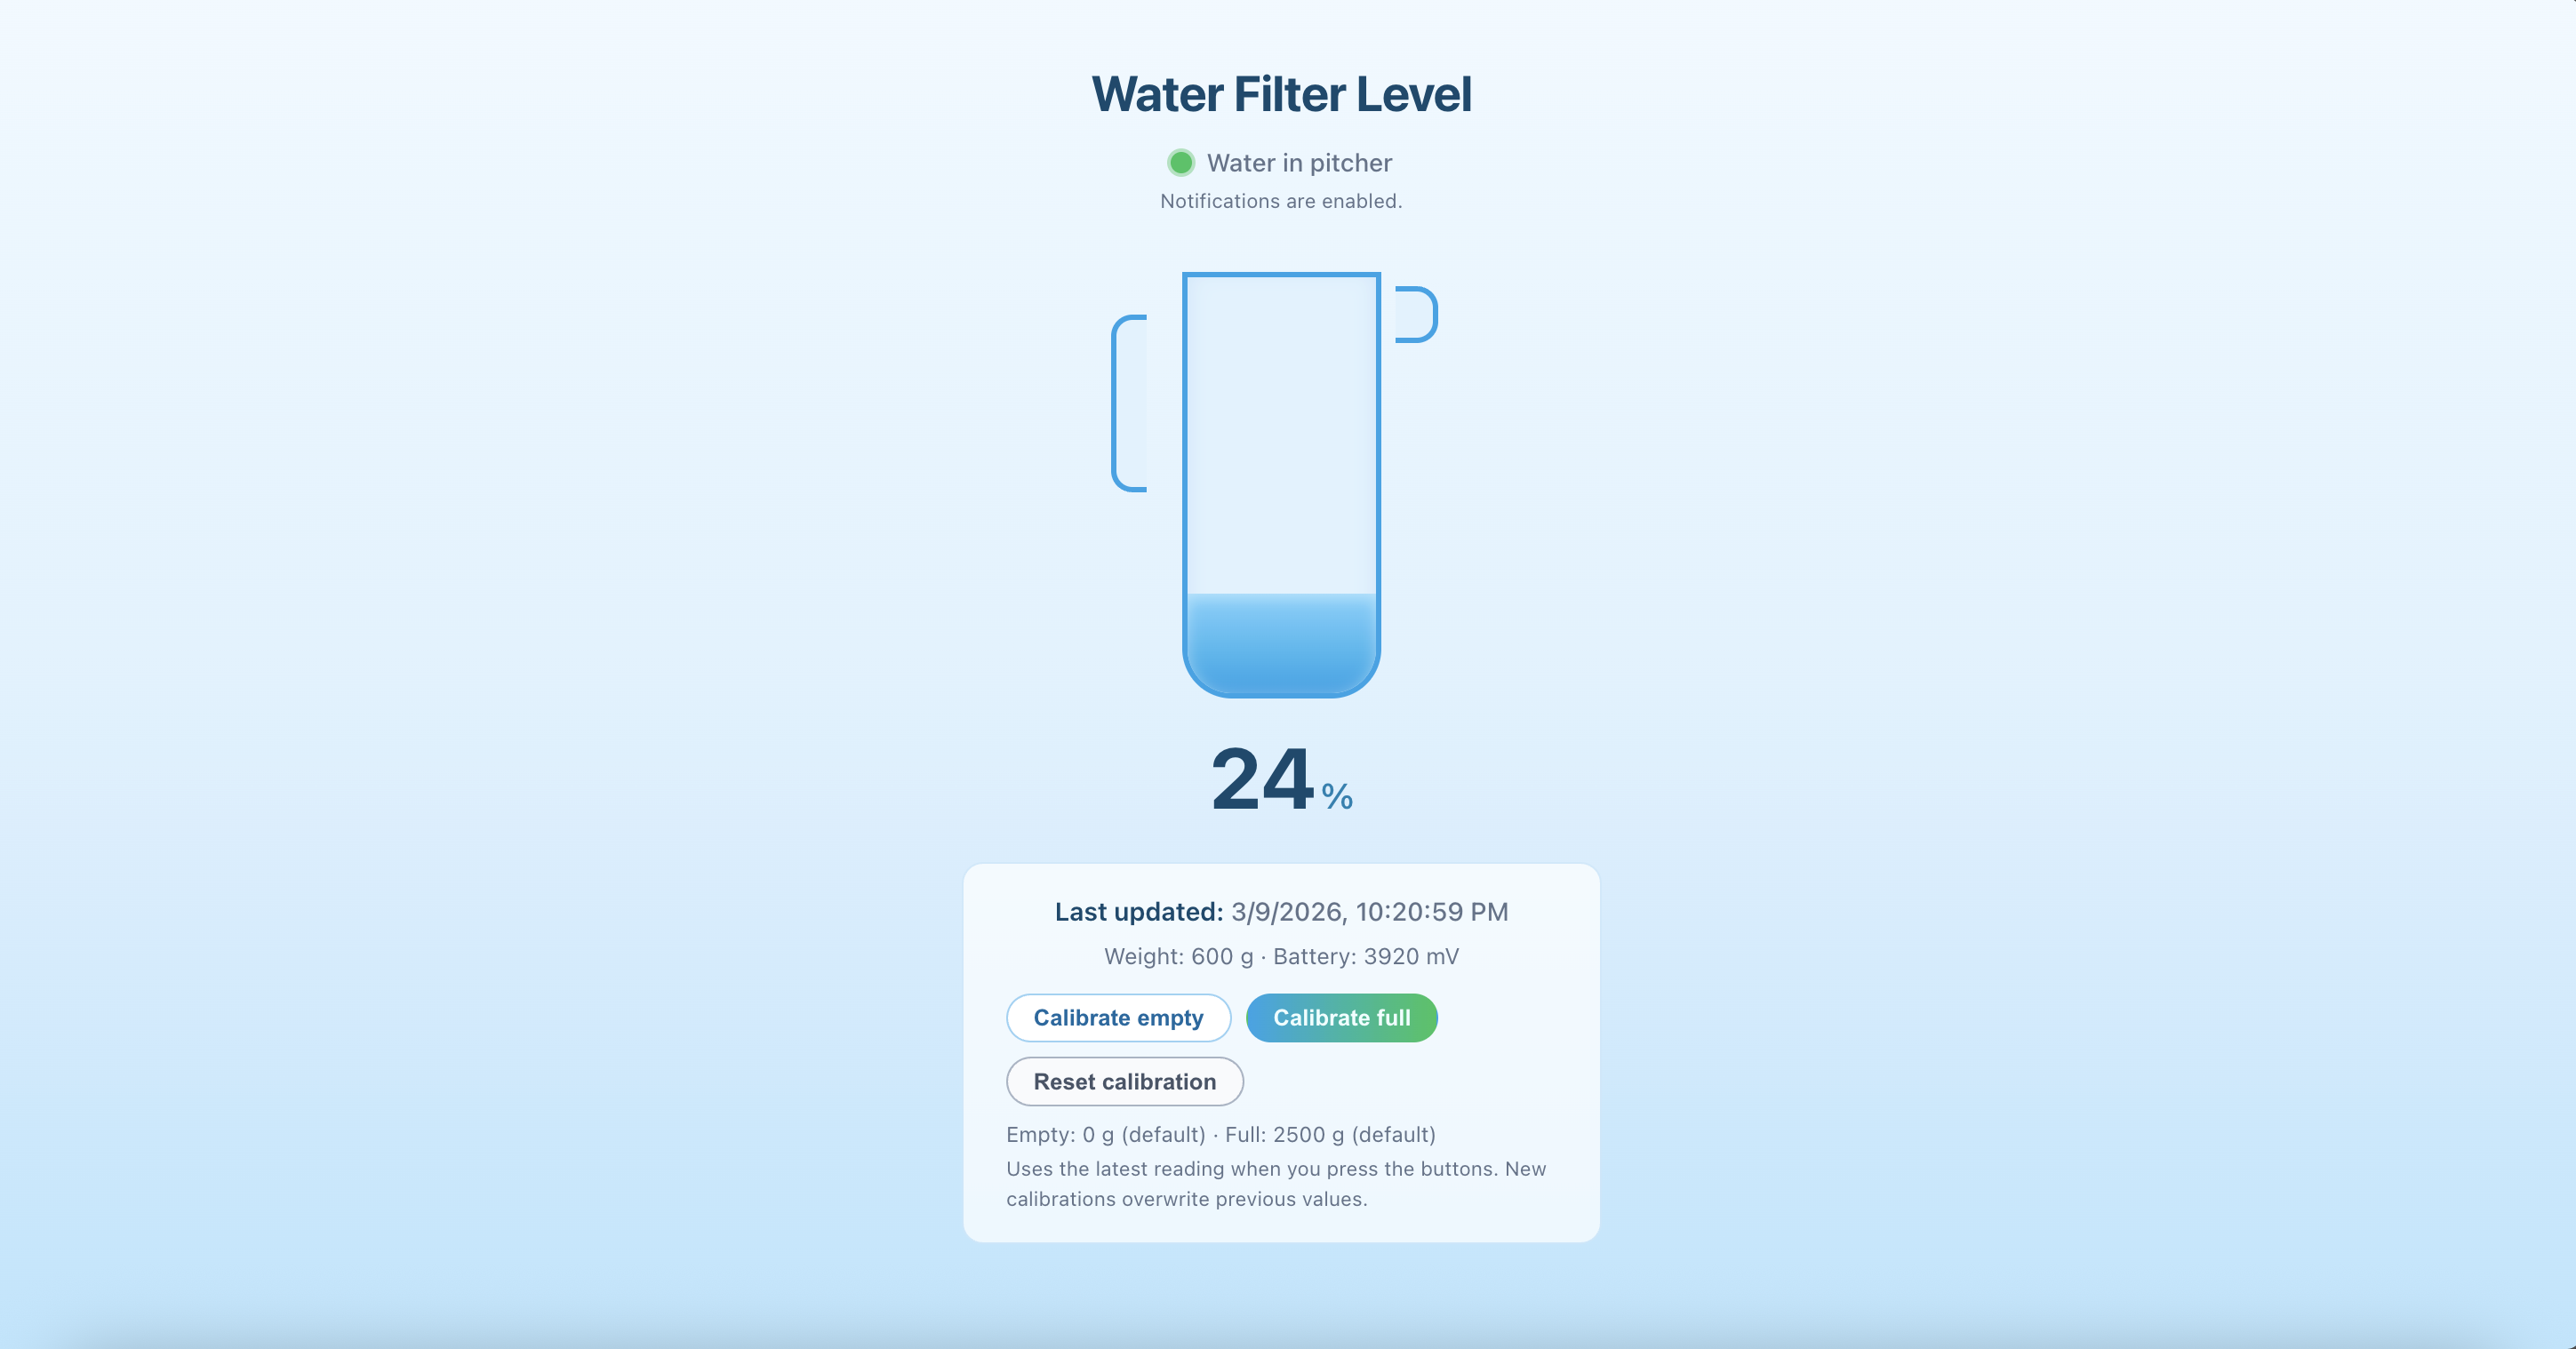
\includegraphics[width=0.75\textwidth]{sections/images/web_app_prototype_notif_enabled.png}
\caption{Web Application with Notifications Enabled}
\label{web_app_prototype_notif_enabled_eval}
\end{center}
\end{figure}
